\documentclass[10pt,tikz]{standalone}
\usepackage{times} % for the font

\usetikzlibrary{matrix}

\newcommand{\texta}{Helpful\\[-1ex] \tiny{(to achieve the objective)}}
\newcommand{\textb}{Harmful\\[-1ex] \tiny{(to achieve the objective)}}
\newcommand{\textcn}{Internal origin\\[-1ex] \tiny{(product\slash company attributes)}}
\newcommand{\textdn}{External origin\\[-1ex] \tiny{(environment\slash market attributes)}}


\begin{document}
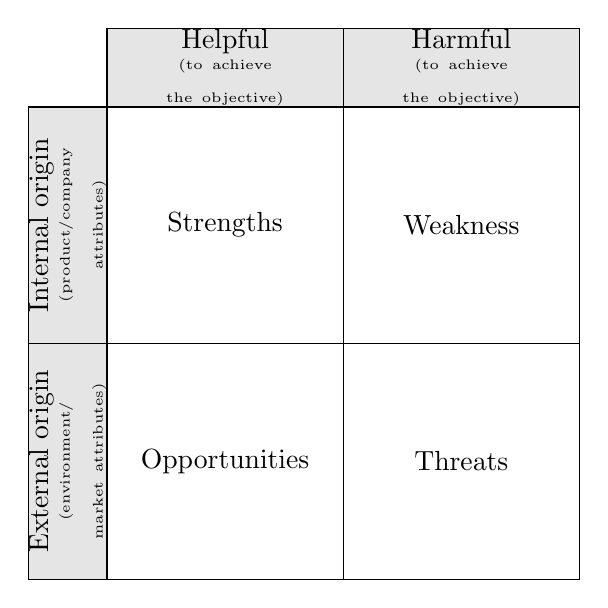
\begin{tikzpicture}[
    any/.style={draw,minimum width=3cm,minimum height=3cm,text width=2.5cm,align=center},
    header/.style={any,minimum height=1cm,fill=black!10},
    leftcol/.style={header,rotate=90}
]

\matrix (SWOT) [matrix of nodes,nodes={any,anchor=center},column sep=-1\pgflinewidth,row sep=-1\pgflinewidth,inner sep=0pt]
{
 &|[header]| {\texta} & |[header]| {\textb} \\
|[leftcol]| {\textcn} & Strengths & Weakness \\
|[leftcol]| {\textdn} & Opportunities & Threats \\
};
\end{tikzpicture}
\end{document}